% utk buat flowchart guna TikZ
\documentclass{minimal}

\usepackage[utf8]{inputenc}
\usepackage{tikz}

\usetikzlibrary{shapes, arrows, positioning, calc}

\begin{document}

Usual way to connect nodes with path

\hfill

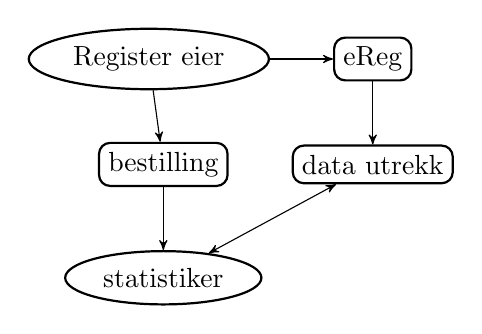
\begin{tikzpicture}
  [
  % block
  block/.style = {rectangle,
    rounded corners,
    draw, thick,
    node distance = 8mm,
    minimum height = 2mm},
  %bulat
  bulat/.style = {ellipse,
    draw, thick, node distance = 8mm,
    minimum height = 5mm},
  % line
  line/.style = {draw, -stealth'},
  ]

  % nodes
  \node [block] (ereg) {eReg};
  \node [bulat, base left= of ereg] (eier) {Register eier};
  \node [block, below= of ereg] (ut) {data utrekk};
  \node [block, left= of ut] (bestil) {bestilling};
  \node [bulat, below= of bestil] (stat) {statistiker};

  % Hvordan får man to noder på lik linje?

  % path
  \path [line] (eier) -- (ereg);
  \path [line] (ereg) -- (ut);
  \path [line] (eier) -- (bestil);
  \path [line] (bestil) -- (stat);
  \path [line, <->, >=stealth'] (ut) -- (stat);

\end{tikzpicture}

\hfill\break
Arrow under ellipse to rectangle with \textbf{\texttt{-|}} as path ID

\hfill

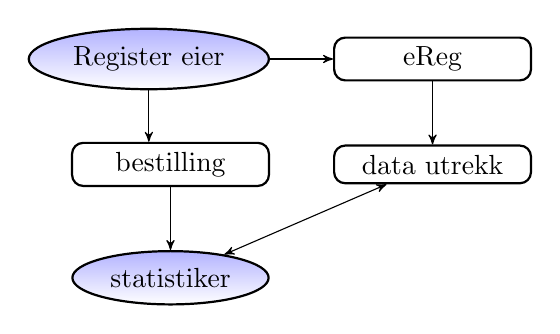
\begin{tikzpicture}
  [
  % block
  block/.style = {rectangle,
    rounded corners,
    draw, thick,
    node distance = 8mm,
    minimum height = 2mm,
    minimum width = 2.5cm},
  %bulat
  bulat/.style = {ellipse,
    draw, thick, node distance = 8mm,
    minimum height = 5mm, top color=blue!30},
  % line
  line/.style = {draw, -stealth'},
  ]

  % nodes
  \node [block] (ereg) {eReg};
  \node [bulat, base left= of ereg] (eier) {Register eier};
  \node [block, below= of ereg] (ut) {data utrekk};
  \node [block, left= of ut] (bestil) {bestilling};
  \node [bulat, below= of bestil] (stat) {statistiker};

  % Hvordan får man to noder på lik linje?

  % path
  \path [line] (eier) -- (ereg);
  \path [line] (ereg) -- (ut);
  \path [line] (eier) -- (bestil.north -| eier.south); % specify intersection
  \path [line] (bestil) -- (stat);
  \path [line, <->, >=stealth'] (ut) -- (stat);

\end{tikzpicture}

\hfill\break
In case someone needs it, this syntax is explained in pgfmanual section "13.3.1 Intersections of Perpendicular Lines".

\texttt{(<p> |- <q>) or (<q> -| <p>)} represent a coordinate at intersection point
between a vertical line passing through coordinate \verb|<p>| and an horizontal
passing through \verb|<q>|. You can use named coordinates like
\texttt{(bestil.north |- eier.south)} that is used here or numeric pairs like in \texttt{(2,1 |- 3,4)}.

\hfill\break
To get alle the nodes aligned for both ellipse and rectangle, the structure starts
from the middle i.e \texttt{bestil} and specify the direction from there. But using
\texttt{below= of stat} as in \verb|positioning package| doesn't locate the
\verb|kode| right below \verb|stat| node.


\begin{tikzpicture}
  [
  block/.style = {rectangle, rounded corners,
    draw, thick, node distance = 1cm, minimum height = 8mm,
    minimum width = 3cm},
  % bulat
  bulat/.style = {ellipse,
    draw, thick, node distance = 1cm,
    minimum height = 5mm, top color=blue!30},
  % line
  line/.style = {draw, -stealth'},
  node distance = 2cm,
  ]

  % nodes
  \node [block] (bestil) {bestilling};
  \node [bulat, above= of bestil] (eier) {Register eier};
  \node [block, right= of bestil] (ut) {utrekk};
  \node [block, above= of ut] (ereg) {eReg};
  % \node [bulat, below= of bestil] (stat) {statistiker};
  \node [block, below = of stat] (kode) {R-koder};


  % path
  \path [line] (eier) -- (bestil);
  \path [line] (ereg) -- (ut);
  \path [line] (eier) -- (ereg);
  %\path [line] (bestil) -- (stat);
  %\path [line] (ut) -- (stat);
  \path (ut) -- node[bulat, below=1.5] (stat) {statistiker} (bestil);
  \path [line] (ut) -- (stat) ;
  \path [line] (bestil) -- (stat);
  \path [line] (stat) -- (kode);

\end{tikzpicture}

\newpage

\hfill\newline Use \verb|calc package| to position node like this: \\
\texttt{\textbackslash node [bulat] (stat) at ($(bestil)!0.5!(ut)+(0,-2)$)
  \{statistiker\};}\newline

\begin{center}
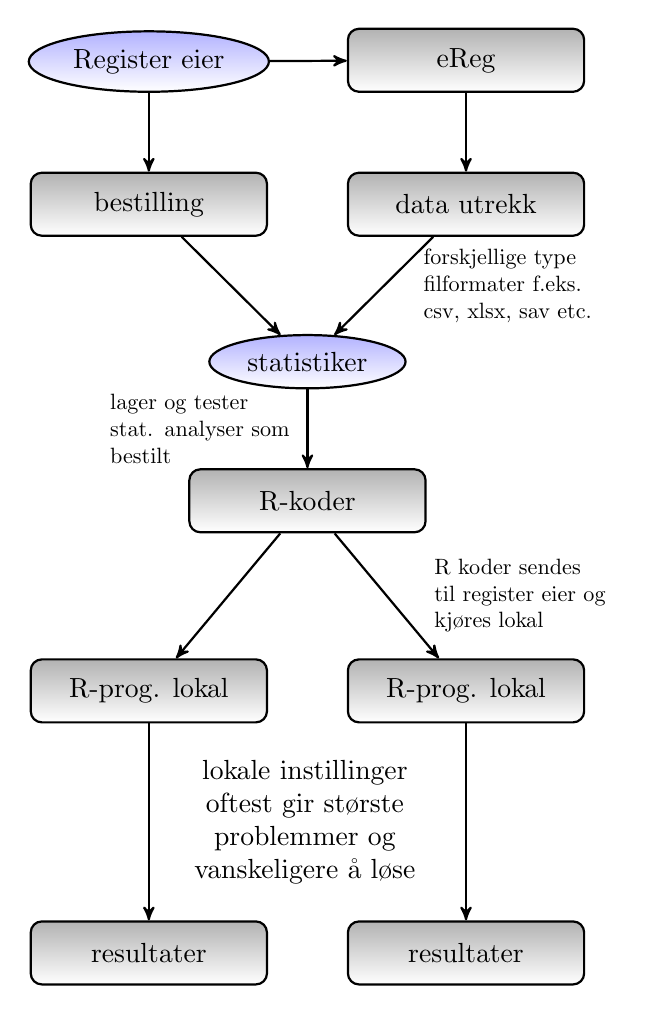
\begin{tikzpicture}
  [
  block/.style = {rectangle, rounded corners, top color=black!30,
    draw, thick, node distance = 1cm, minimum height = 8mm,
    minimum width = 3cm},
  % bulat
  bulat/.style = {ellipse,
    draw, thick, node distance = 1cm,
    minimum height = 5mm, top color=blue!30},
  % line
  line/.style = {draw, -stealth', thick},
  node distance = 2cm,
  ]

  % nodes
  \node [block] (bestil) {bestilling};
  \node [bulat, above= of bestil] (eier) {Register eier};
  \node [block, right= of bestil] (ut) {data utrekk};
  \node [block, above= of ut] (ereg) {eReg};
  % calc pkg between 'bestil' and 'ut' and downward at coordinat 0pt,-2pt
  \node [bulat] (stat) at ($(bestil)!0.5!(ut)+(0,-2)$) {statistiker};
  \node [block, below = of stat] (kode) {R-koder};
  % buat center coordinate utk menetapkan posisi'r1' dan 'r2
  \coordinate [below = of kode] (center) {};
  \node [block, left =.5 of center] (r1) {R-prog. lokal};
  \node [block, right =.5 of center] (r2) {R-prog. lokal};
  \node [block, below = 2.5 of r1] (rest1) {resultater};
  \node [block, below = 2.5 of r2] (rest2) {resultater};

  % path
  \path [line] (eier) -- (bestil);
  \path [line] (ereg) -- (ut);
  \path [line] (eier) -- (ereg);
  \path [line] (ut) -- node [right = .4, scale=.8, text width = 3cm]
  {forskjellige type \\ filformater f.eks. csv, xlsx, sav etc.} (stat) ;
  \path [line] (bestil) -- (stat);
  \path [line] (stat) -- node [left, scale=.8, text width=3cm]
  {lager og tester stat. analyser som bestilt}(kode);
  % % tekst
  % \path [line] (kode) -- node [left, scale =.8, text width = 3cm]
  % {R koder sendes til register eier og kjøres lokal} (r1);
  \path [line] (kode) -- (r1);
  % tekst inkludert
  \path [line] (kode) -- node [right = .5, scale =.8, text width = 3cm]
  {R koder sendes til register eier og kjøres lokal} (r2);
  % tekst lokasjon og 'text width' kontrollere størrelse for å legge tekstene
  \path [line] (r1) -- node [right = 1mm, text width = 3.5cm, align=center]
  {lokale instillinger \\ oftest gir største \\ problemmer og vanskeligere å løse} (rest1);
  \path [line] (r2) -- (rest2);

\end{tikzpicture}
\end{center}

\end{document}
